\section{非凸目标与鞍点}
\label{sec:opt-smooth-nonconvex}

前两节的保证在非凸目标上只剩下“梯度变小”。本节研究这句话究竟说了什么：下降方法可能停在哪些点，梯度小与到达局部最小点相差多远；以及在已有梯度和曲率信息的前提下，怎样主动离开那些不是最小点的驻点。全节分析离散迭代，连续时间的梯度流不能代替离散算法的结论。

\subsection{驻点残差与负曲率下降}
\label{sec:opt-smooth-negative-curvature}

\paragraph{梯度趋零说明了什么}
第~\ref{chap:optimization}章给出了内点处的最优条件：局部最小点必须满足$\nabla f=\bm0$与$\nabla^2f\succeq\bm0$；驻点处$\nabla^2f\succ\bm0$则足以保证严格局部最小。定理~\ref{thm:opt-smooth-gd-nonconvex}保证的是$\nabla f(\bm x^{(t)})\to\bm0$，这与“迭代收敛到驻点”之间还隔着两步。第一，梯度趋零不意味着迭代有界：$f(x)=e^{-x}$在$[0,\infty)$上下有界且$L=1$光滑，从$x^{(0)}=0$用$\eta=1$出发，迭代单调右移、梯度趋于零，却根本没有驻点可以趋近。第二，若迭代有界，由梯度的连续性，每个聚点都是驻点；但聚点可能不止一个，仅凭梯度趋零推不出整个序列收敛到某一点。所以“返回梯度小的点”这句话，只对应“近似一阶驻点”。

\paragraph{驻点的种类}
驻点处若$\nabla^2f$有负特征值，就称为\term{严格鞍点}（strict saddle point）。这个名称约定也覆盖局部最大点，因为它们同样有负曲率方向；关键在于负曲率提供了离开的方向。为了区分“梯度小”的点里哪些可能接近局部最小点，引入双容差：若
\[
  \lVert\nabla f(\bm x)\rVert_2\leq\varepsilon_g,\qquad\lambda_{\min}\bigl(\nabla^2f(\bm x)\bigr)\geq-\varepsilon_H,
\]
就称$\bm x$为\term{近似二阶驻点}（approximate second-order stationary point）。它排除了曲率明显为负的鞍点，但仍不是局部最小性的充分条件。$f(x_1,x_2)=x_1^4-x_2^4$在原点处梯度和Hessian都为零，满足任意容差下的近似二阶条件，却是鞍点：沿$x_1$轴目标为正、沿$x_2$轴为负。高阶平坦的鞍点用一阶和二阶信息都看不出来。

\paragraph{沿负曲率方向下降}
在鞍点附近，梯度很小，梯度步几乎不动；但若已经知道一个负曲率方向，就能用二阶信息得到可量化的下降。设单位向量$\bm v$满足$\bm v^\top\nabla^2f(\bm x)\bm v\leq-\gamma<0$，称为\term{负曲率方向}（negative curvature direction）。必要时把$\bm v$换成$-\bm v$，使$\langle\nabla f(\bm x),\bm v\rangle\leq0$。若Hessian在包含$[\bm x,\bm x+\alpha\bm v]$的凸区域上$M$-Lipschitz，由立方正则化小节的三阶余项界，
\[
  f(\bm x+\alpha\bm v)\leq f(\bm x)+\alpha\langle\nabla f(\bm x),\bm v\rangle+\frac{\alpha^2}2\bm v^\top\nabla^2f(\bm x)\bm v+\frac M6\alpha^3
  \leq f(\bm x)-\frac\gamma2\alpha^2+\frac M6\alpha^3 .
\]
右边在$\alpha=2\gamma/M$处最小，给出
\begin{equation}
\label{eq:opt-smooth-negative-curvature-decrease}
  f\Bigl(\bm x+\frac{2\gamma}M\bm v\Bigr)\leq f(\bm x)-\frac{2\gamma^3}{3M^2}.
\end{equation}
下降量只取决于负曲率的大小和Hessian的变化速度，与梯度多小无关，正好补上梯度步在鞍点附近的不足。例如$f(\bm x)=\tfrac14x_1^4-\tfrac12x_1^2+\tfrac12x_2^2$在原点有$\nabla^2f=\operatorname{diag}(-1,1)$，取$\bm v=(1,0)^\top$、$\gamma=1$；在$|x_1|\leq1$上$\partial^3f/\partial x_1^3=6x_1$，$M=6$。步长$\alpha=1/3$给出$f(1/3,0)\approx-0.0525$，不高于界$-2/(3\cdot36)\approx-0.0185$。

\paragraph{检测负曲率的代价}
式~\eqref{eq:opt-smooth-negative-curvature-decrease}的前提是手里真有一个负曲率方向。寻找它要计算Hessian的最小特征值或其近似，例如用Lanczos方法，每步一次Hessian向量积；检测本身有误差，所得的$\gamma$只是Rayleigh商的估计，应先核实$\bm v^\top\nabla^2f(\bm x)\bm v$，再用原目标检验位移。这些计算都应计入算法的成本。用正定近似代替真实Hessian是检测不到负曲率的：BFGS矩阵、修正牛顿的$\bm H+\bm E$按构造总是正定的，它们没有负特征值不说明真实Hessian没有；上一节也说明，Newton--CG的内层只看Krylov子空间，同样可能漏掉负曲率。

\subsection{扰动与逃离鞍点}
\label{sec:opt-smooth-perturbed}

不计算Hessian，只用梯度，能否离开鞍点？先看梯度下降在鞍点附近怎样运动。对上一小节的例子，梯度下降的两个坐标各自演化：
\[
  x_1^{(t+1)}=x_1^{(t)}+\eta\bigl(x_1^{(t)}-(x_1^{(t)})^3\bigr),\qquad x_2^{(t+1)}=(1-\eta)x_2^{(t)} .
\]
在原点附近$x_1$每步约乘以$1+\eta$，$x_2$每步乘以$1-\eta$。从$x_1^{(0)}=0$出发，$x_1$永远为零，迭代沿$x_2$轴收敛到鞍点；这条轴就是鞍点的稳定流形。只要$x_1^{(0)}\neq0$，哪怕非常小，$x_1$就会按几何级数放大，迭代最终离开鞍点、落入某个最小点$(\pm1,0)$的吸引域。图~\ref{fig:opt-smooth-saddle-escape}取$\eta=0.2$：从$(10^{-3},1.5)^\top$出发的路径先沿$x_2$轴下滑，在鞍点附近停留十余步，到第$35$步$x_1$才超过$0.5$，随后落到最小点$(1,0)$；它在徘徊处梯度很小，若此时按梯度容差停止，就会把鞍点附近的点当作结果返回。

\begin{figure*}[htbp]
  \centering
  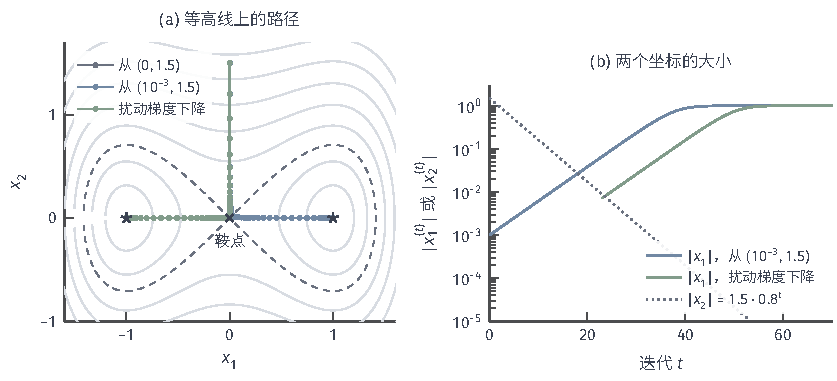
\includegraphics[width=141.7mm]{figures/03-optimization-evolution-and-signals/01-optimization/tikz/c3-saddle-escape/figure.pdf}
  \caption{目标$f(\bm x)=\tfrac14x_1^4-\tfrac12x_1^2+\tfrac12x_2^2$上步长$\eta=0.2$的梯度下降，叉号为原点处的严格鞍点，星号为最小点$(\pm1,0)$，灰色虚线是零等值线。(a) 从$(0,1.5)^\top$出发（灰）沿稳定流形收敛到鞍点；从$(10^{-3},1.5)^\top$出发（蓝）先接近鞍点再离开；扰动梯度下降（绿）从$(0,1.5)^\top$出发，在梯度降到$10^{-2}$时（第23步）加入半径$10^{-2}$内的均匀扰动，随后离开。(b) 对数坐标下$|x_1^{(t)}|$与$|x_2^{(t)}|$：负曲率坐标每步约放大$1.2$倍（直线上升），正曲率坐标每步乘以$0.8$。}
  \label{fig:opt-smooth-saddle-escape}
\end{figure*}

\paragraph{普通梯度下降的渐近避鞍}
上面的例子说明，收敛到严格鞍点需要初值恰好落在一个“零测”的稳定流形上。这一观察有严格的版本：设$f$二阶连续可微、梯度全局$L$-Lipschitz，步长$0<\eta<1/L$，初值服从对Lebesgue测度绝对连续的分布，则对每个严格鞍点，梯度下降收敛到它的概率为零\cite{lee2016gradient}。这里的随机性只来自初值，之后的迭代完全确定。结论有三个限度。它是渐近的，不说明离开需要多少步，图中蓝色路径若初值更接近稳定流形，徘徊时间会按$\log(1/|x_1^{(0)}|)$增长。它只排除收敛到严格鞍点，要说“几乎必然收敛到局部最小点”，还需迭代本身收敛、所有非最小驻点都是严格鞍点等额外条件。它针对固定步长的梯度下降，不能直接搬到回溯步长、动量或随机梯度。

\paragraph{扰动梯度下降}
要得到有限步的保证，可以在可疑区域主动加一点随机扰动，把迭代推离稳定流形。\term{扰动梯度下降}（perturbed gradient descent）的骨架如下\cite{jin2017escape}。

\begin{algorithm}[扰动梯度下降的骨架]
\label{alg:opt-smooth-pgd}
\begin{algorithmic}[1]
\Require 初值$\bm x^{(0)}$，步长$\eta$，梯度阈值$g_{\mathrm{th}}$，扰动半径$r$，观察窗口长度$t_{\mathrm{th}}$，下降阈值$f_{\mathrm{th}}$
\Ensure 返回点
\State $t_{\mathrm{p}}\gets-\infty$（上次扰动的时刻）
\For{$t=0,1,2,\dots$}
  \If{$\lVert\nabla f(\bm x^{(t)})\rVert_2\leq g_{\mathrm{th}}$ 且 $t-t_{\mathrm p}>t_{\mathrm{th}}$}
    \State 保存基点$\tilde{\bm x}\gets\bm x^{(t)}$及$f(\tilde{\bm x})$，$t_{\mathrm p}\gets t$
    \State $\bm x^{(t)}\gets\tilde{\bm x}+\bm\xi$，$\bm\xi$在半径$r$的球内均匀抽取
  \EndIf
  \If{$t-t_{\mathrm p}=t_{\mathrm{th}}$ 且 $f(\bm x^{(t)})>f(\tilde{\bm x})-f_{\mathrm{th}}$}
    \State \Return $\tilde{\bm x}$ \Comment{窗口内没有足够下降，基点视为近似二阶驻点}
  \EndIf
  \State $\bm x^{(t+1)}\gets\bm x^{(t)}-\eta\nabla f(\bm x^{(t)})$
\EndFor
\end{algorithmic}
\end{algorithm}

算法的逻辑是一个检验：梯度小时，在基点周围随机挪一点，再跑一段普通梯度下降；若基点附近有明显的负曲率，扰动几乎必然带有该方向的分量，这个分量在窗口内被放大，目标下降至少$f_{\mathrm{th}}$；若窗口结束时没有这么多下降，就推断基点附近没有明显的负曲率，返回基点。扰动不是“随便加噪声”：它只在规定条件下触发，半径、窗口长度和阈值都由$L$、$M$、目标精度$\varepsilon$、失败概率$\delta$与初始目标差联合确定，返回的是保存的基点而不是扰动后的点。图~\ref{fig:opt-smooth-saddle-escape}中的绿色路径从稳定流形上出发，普通梯度下降会停在鞍点；第$23$步的扰动把$x_1$从$0$推到约$-0.007$，之后与蓝色路径一样离开，只是落向另一个最小点$(-1,0)$。

\paragraph{有限步保证与它的含义}
在$f$二阶连续可微、梯度$L$-Lipschitz、Hessian $M$-Lipschitz、$f$下有界等条件下，适当选取参数的扰动梯度下降以至少$1-\delta$的概率返回满足
\[
  \lVert\nabla f(\bm x)\rVert_2\leq\varepsilon,\qquad\lambda_{\min}\bigl(\nabla^2f(\bm x)\bigr)\geq-\sqrt{M\varepsilon}
\]
的点，所需梯度计算次数为$\tilde O\bigl(L(f(\bm x^{(0)})-f_{\inf})/\varepsilon^2\bigr)$，其中$\tilde O$隐去了关于$d$、$1/\delta$等的对数因子\cite{jin2017escape}。与定理~\ref{thm:opt-smooth-gd-nonconvex}相比，梯度计算次数只多了对数因子，却额外控制了负曲率。与上一小节的普通梯度下降结论对照：前者是对初值随机性的渐近陈述，后者是对算法内部随机扰动的有限步、高概率陈述，两者的条件和结论都不同。最后要记住，近似二阶驻点仍不等于局部最小点（高阶平坦的鞍点可以满足它），更不等于全局最小点：目标若有不好的局部最小点，任何局部方法都可能停在那里，要排除这种情况，需要对目标的整体形状另作分析。
